\documentclass[11pt]{article}
\linespread{1.5}

\usepackage{preamble}
\usepackage[spanish,es-tabla]{babel}


\begin{document}

\pagenumbering{gobble}
{

% Title
\subfile{title}

% Abstract
% \subfile{abstract}

\newpage

\hypersetup{linkcolor=black}

\renewcommand\contentsname{Índice de contenido}
\tableofcontents

\clearpage

% List of codes
\tcblistof[\section*]{code}{Índice de código}
% List of theorems
% \tcblistof[\section*]{theorem}{\theoListTitle}
% List of figures
\renewcommand\listfigurename{Índice de figuras}
\listoffigures
% List of tables
\renewcommand\listtablename{Índice de tablas}
\listoftables

}
\clearpage
\pagenumbering{arabic}

% ACRONYMS
\printglossary[type=\acronymtype, title=Glosario de acrónimos, nonumberlist]
\label{sec:acronyms}

% ------------------------- CONTENT ------------------------- %

\section{Introducción}

Las micotoxinas son toxinas naturales derivadas del metabolismo secundario de mohos micotoxigénicos, que se pueden encontrar en alimentos y materias primas. Una de ellas,
el \acrfull{don}, se encuentra en el campo predominantemente en granos de cereales como el trigo. Por este motivo, el deoxinivalenol se encuentra frecuentemente en
alimentos a base de cereales lo que, unido a la elevada ingesta de trigo típica de la dieta española, hace que la exposición de la población sea significativa. En los años
en que la meteorología es especialmente adversa los cultivos de todo el mundo muestran altos niveles de contaminación. Además, en los últimos años existe una creciente
evidencia de un aumento en la incidencia de micotoxinas como resultado del cambio climático.

Actualmente, las empresas procesadoras de cereales basan su autocontrol en el análisis de muestras de un determinado número de lotes mediante técnicas inmunocromatográficas
rápidas, de forma que se rechazan los lotes no conformes. Los lotes que, una vez analizados, superan el límite legal \(1250 \mu g/kg\), en general, se desvían íntegramente
a la alimentación animal. En el sector de la alimentación animal, el problema se hace más evidente, ya que el consumo de piensos contaminados se evidencia en una menor
ganancia de peso del ganado y el impacto en otros parámetros productivos y de salud animal.


\subsection{Motivación}

El desafío que se plantea se centra en las operaciones de selección y clasificación de granos mediante \acrfull{nir-hsi}, previas a la transformación, que
de ser efectivas podrían aplicarse a lotes que superen los \(1250 \mu g/kg\), con la intención de devolver dichos lotes a la cadena alimentaria, una vez se ha separado
la fracción más contaminada. De esta manera, la fracción que podría destinarse al consumo humano sería posiblemente mayoritaria, y el sistema de producción de alimentos,
en su conjunto, más sostenible. Como consecuencia, las motivaciones son las contribuciones a la seguridad alimentaria y ambiental con protección a través de nuevas 
tecnologías que permitan aplicaciones avanzadas para la agricultura y los sistemas alimentarios, a evitar pérdidas y derroche alimentario; pues los métodos actuales de 
control de calidad no permiten un control óptimo. La inspección por \gls{nir-hsi} puede permitir superar este problema.


\subsection{Objetivos}

Nuestro objetivo como parte del proyecto es claro, construir un modelo de predicción robusto con los datos que tenemos, la validación de los modelos generados y la técnica en
condiciones de laboratorio con un número suficiente de muestras reales y el desarrollo de software para la detección en tiempo real de granos contaminados. 

Para ello, hemos separado esta tarea en diferentes pasos discernibles. 

\begin{enumerate}
    \item Entender los datos de los resultados de laboratorio.
    \item Entender el existente proceso de análisis de imágenes hiperespectrales.
    \item Tratar de mejorar el actual proceso de análisis de las imágenes.
    \item Entender el actual proceso de entranamiento y análisis de modelos de \gls{ml}.
    \item Tratar de mejorar el preprocesado de los datos, tanto como el entrenamiento de nuevos modelos para tratar de obtener mejores resultados.
    \item Entrenar buenos modelos de \gls{ml} que, según las imágenes hiperespectrales, sean capaces de predecir si un grano está contaminado. 
    \item Una vez entrenados los modelos básicos, tratar de ajustarlos a los datos con \textit{Hyperparameter tuning}.
    \item Añadir nuevos modos de ejecución del programa para emular la carga continua de imágenes que habría en un caso de uso real, además de prepararlo para que se 
    pueda ejecutar por un tiempo indefinido como en un caso real, guardando los resultados de las predicciones.
\end{enumerate}

\subsection{Estructura del documento}


\section{Análisis del problema}

El principal problema que nos concierne es la detección y separación del grano contaminado de la corriente de cereal circulando por los transportadores. Para solucionarlo,
la propuesta de sistema a implementar consiste en la instalación de cámaras infrarojas en la línea de procesado, capaces de captar las imágenes hiperespectrales de la
corriente. De manera que utilizando nuestro modelo previamente calibrado, se detecte cuáles son los granos más contaminados y se puedan separar por una corriente de aire. 
Podemos ver un esquema del sistema en la \textit{imagen\ \ref{fig:detection-system}}.

\begin{figure}[!h]
    \centering
    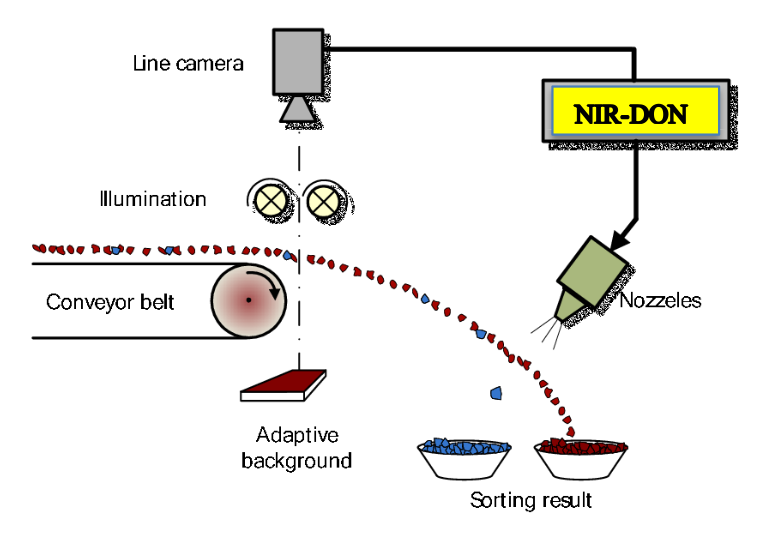
\includegraphics[width=0.7\linewidth]{media/images/esquema-del-sistema.png}
    \caption{Esquema del sistema de detección y filtrado de granos contaminados}\ \label{fig:detection-system}
\end{figure}


\subsection{NIR-HSI}


\gls{nir-hsi} es una tecnología rápida, no destructiva y precisa que nos permite hacer inspecciones de calidad, la cual ha demostrado su potencial en los últimos años\ \cite{Applicat5:online}. 
Es una técnica de imagen química basada en la espectroscopia de reflectancia (la luz reflejada por los materiales), la cual es capaz de caracterizar compuestos orgánicos y algunos minerales\ \cite{NIRHyper23:online}. Este método puede resultar mucho más directo, pues es rápido y no requiere análisis químico; barato, por los mismos motivos; y preciso, pues permite analizar los granos individualmente y no en lote; que el análisis químico.

Como hemos comentado en la introducción, nuestro objetivo es conseguir un modelo que, utilizando \gls{nir-hsi}, prediga lo mejor posible qué granos de una \gls{imagen hiperespectral} contienen granos contaminados con \acrshort{don}. Para ello, partimos con una base de datos de imágenes hiperespectrales con formato \acrshort{bil}, las cuales simulan las imágenes tomadas en la cadena de producción y de las cuáles podemos extraer la información de los píxeles que forman los granos.
Los archivos con formato \acrshort{bil} albergan los datos hiperespectrales de una imagen, como podemos ver en la \textit{figura \ref{fig:bil-example}}. Es decir, para las diferentes bandas especificadas, contiene la información de cada píxel que forma la imagen. Para ello, hace uso de otro archivo complementario con formato \textit{bil.hdr} que brinda información sobre este, como las diferentes bandas (frecuencias, en nuestro caso son 168) presentes en la imagen, entre otros. Una vez sabemos qué formato tienen los datos, podemos leer los archivos \acrshort{bil} que tenemos y formar un \acrshort{csv} con los datos centralizados para que nos sea más fácil trabajar con ellos. Para no tener un archivo demasiado grande, hemos desechado los píxeles que forman parte del `fondo' negro de la imagen, para determinar si un píxel es fondo, se hace la media de todos los valores de las reflectancias para ese píxel y si no pasa un umbral trivial, lo consideramos parte del fondo.

Una vez tenemos el \acrshort{dataset} con los datos de cada píxel, podemos generar un nuevo \acrshort{dataset} que agrupe los píxeles en grupos, o granos. De esta forma, podemos añadir un nuevo filtro que consista en que los granos deben de tener un tamaño mínimo (en píxeles), es decir, podemos desechar los granos que sean demasiado pequeños ya que probablemente sea ruido en la imagen. De esta forma, agruparíamos \textit{N} filas de datos de píxeles, en tan solo una fila conservando la media de cada columna.

\begin{figure}[!ht]
    \centering
    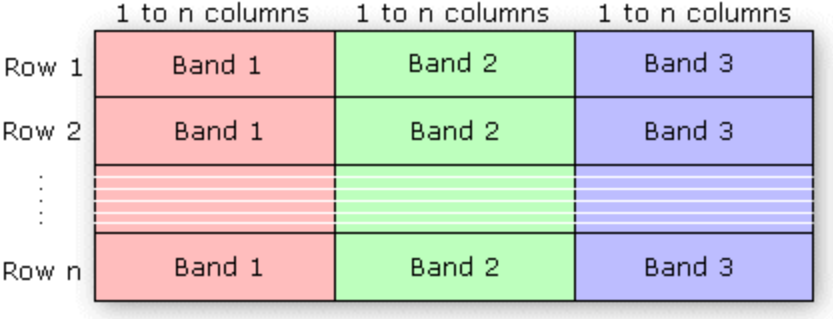
\includegraphics[width=0.7\linewidth]{media/images/bil.png}
    \caption{Formato de los datos en un archivo \acrshort{bil}. Fuente \cite{Archivos82:online}}\ \label{fig:bil-example}
\end{figure}

Por otro lado, tenemos una base de datos con el estado de contaminación de estos mismos granos. A partir de ahora utilizaremos los términos contaminación y etiqueta como sinónimos a la hora de referirnos a los granos.


\subsection{Contaminación del grano}\ \label{sec:separacion}

El valor de contaminación \acrshort{don} de una muestra se obtiene, como hemos comentado anteriormente, realizando un análisis químico por lotes. Este análisis nos devuelve el valor de la concentración de \acrshort{don} en el lote, de modo que si supera los \(1250\ \mu g/kg\), por ley, la muestra se considera contaminada. Sabiendo esto, previamente en laboratorio se ha realizado un análisis de los granos que forman las imágenes \acrshort{bil} que tenemos y, por lo tanto, además de los datos hiperespectrales, sabemos el nivel de contaminación que posee cada grano y lo podemos agregar como columna en el \acrshort{csv} que tenemos.


Al ser el valor de contaminación el que queremos predecir, a partir de ahora utilizaremos los términos contaminación y etiqueta como sinónimos. Además agregaremos otra columna, también de contaminación, la cual será \textit{booleana}, en lugar de un valor contínuo, y nos indicará si el valor concentración de ese grano supera el umbral legal comentado anteriormente. De esta forma, podemos plantear el problema tanto por regresión como por clasificación, 


\subsection{Análisis del mercado potencial}






\section{Marco teórico, conceptos clave del ML}

\begin{quote}
    `\gls{ml}: the use and development of computer systems that are able to learn and adapt without following explicit instructions, by using algorithms and statistical models to analyse and draw inferences from patterns in data'\ \cite{machinel18:online}
\end{quote}

Es decir, un sistema que es capaz de inferir patrones de unos datos y realizar predicciones sobre nuevos datos a raíz de los patrones encontrados. 


\subsection{Tipos de aprendizaje y modelos}

Hay cuatro tipos de aprendizaje en el ML:\@ supervisado, no supervisado, semi-supervisado y de refuerzo\ \cite{homl56}.

Como parte de nuestros datos están etiquetados, podemos utilizar tanto el aprendizaje supervisado como el semi-supervisado. En un sistema supervisado se requiere que todos los datos estén etiquetados con la categoría deseada, en nuestro caso la contaminación. Sin embargo, para el semi-supervisado no es necesario que todos los datos estén etiquetados, pues utilizan tanto los datos etiquetados como los que no (datos parcialmente etiquetados) para tratar de generalizar mejor\ \cite{homl56}.

No utilizaremos el no supervisado, pues consiste en un conjunto de técnicas utilizadas para agrupar automáticamente datos no etiquetados a base de similitudes sin tener supervisión previa. El objetivo es que los datos dentro de un mismo grupo sean más similares entre sí que con los otros grupos\ \cite{Clustera13:online}. Sin embargo, como tenemos una cantidad más o menos considerable de información etiquetada, no nos hace falta.

Tampoco utilizaremos el aprendizaje por refuerzo, pues no se encuentra implementado dentro de la librería que utilizamos \textit{\href{https://scikit-learn.org/stable/}{sklearn}} y tampoco está dentro de los objetivos del proyecto.


\subsection{Fases del desarrollo de un proyecto de ML}

Nuestro proyecto ha tenido las fases que nombramos a continuación:

\begin{enumerate}
    \item Obtención de datos (\textit{apartado\ \ref{sec:obtencion}})
        \begin{enumerate}
            \item Recolección de información de los \acrshort{bil}.
        \end{enumerate}
    \item Preparación de datos (\textit{apartado\ \ref{sec:preprocesado}})
        \begin{enumerate}
            \item Selección de métodos de preprocesado
        \end{enumerate}
    \item Entrenamiento de los modelos (\textit{apartado\ \ref{sec:entrenamiento}})
        \begin{enumerate}
            \item Entrenamiento `básico' de modelos
            \item Selección y refinamiento
        \end{enumerate}
    \item Evaluación de resultados
        
    \item Monitoreo de los modelos
\end{enumerate}

Podemos generalizar los procesos de un proyecto de \gls{ml} meidnate el esquema de la \textit{Figura\ \ref{fig:ml-development-cycle}}. Cabe destacar que el proceso de entrenar un modelo de \gls{ml}, como bien muestra la imagen, es un proceso cíclico en búsqueda de mejores resultados a base de probar metodologías distintas, añadir pasos, el cambio de requisitos, etc.

\begin{figure}[!htb]
    \centering
    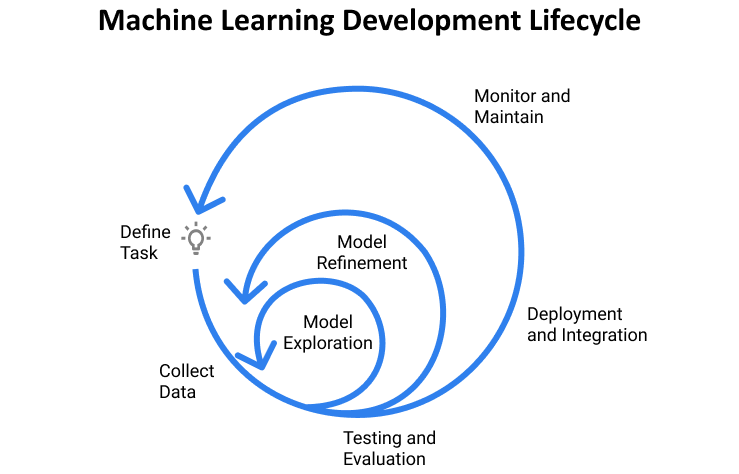
\includegraphics[width=\linewidth]{media/images/ml-development-cycle.png}
    \caption{Esquema del proceso del desarrollo de un proyecto de \gls{ml}, fuente\ \cite{Organizi22:online}}\ \label{fig:ml-development-cycle}
\end{figure}


\subsection{Métricas de evaluación de modelos}

Antes de continuar con el entrenamiento de modelos, su mejora y la selección de pasos del preprocesado; necesitamos algún tipo de métrica para evaluar y comparar los resultados. A continuación, explicaremos las que hemos utilizado para los diferentes tipos de modelos.

\subsubsection{Clasificación supervisada y semi-supervisada}\ \label{sec:classification-metrics}

Primeramente, explicaremos las partes de una matriz de confusión como la que podemos ver en la \textit{Figura\ \ref{fig:confusion-matrix-example}}. Podemos ver que tiene cuatro partes:

\begin{itemize}
    \item \textit{True Positive (tp)}, las muestras que el modelo clasifica como positivas que realmente son positivas.
    \item \textit{False Positive (fp)}, las muestras que el modelo clasifica como positivas que realmente son negativas.
    \item \textit{True Negative (tn)}, las muestras que el modelo clasifica como negativas que realmente son negativas.
    \item \textit{False Negative (fn)}, las muestras que el modelo clasifica como negativas que realmente son positivas.
\end{itemize}

Estos cuatro valores son la base del resto de métricas que comentaremos a continuación.

\begin{figure}[!ht]
    \centering
    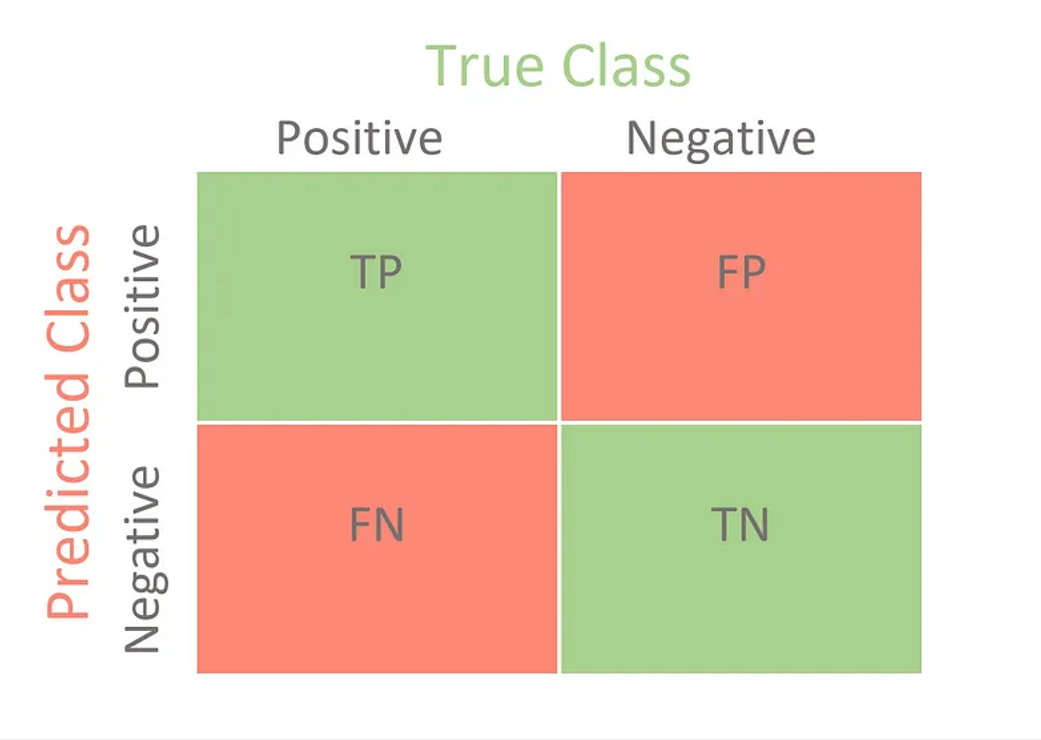
\includegraphics[width=0.7\linewidth]{media/images/confusion-matrix-example.png}
    \caption{Ejemplo de matriz de confusión, fuente\ \cite{Confusio71:online}}\ \label{fig:confusion-matrix-example}
\end{figure}

Antes de continuar con las métricas que compararemos, comentaremos también otras más básicas que son utilizadas para calcular las que utilizaremos\ \cite{Precisio23:online}.
\\ \textit{\textbf{Sensitivity}} permite saber la probabilidad de que una predicción positiva sea realmente positiva.
    \begin{equation}
        sensitivity=tp/(tp+fn)
    \end{equation}
\textit{\textbf{Specificity}} permite saber la probabilidad de que una predicción negativa sea realmente negativa.
\begin{equation}
        specificity=tn/(tn+fp)
    \end{equation}
\textit{\textbf{Recall}} indica la capacidad del modelo para encontrar todas las muestras positivas. 
    \begin{equation}
        recall=tp/(tp+fn)
    \end{equation}
\textit{\textbf{Precision}} indica la precisión de las predicciones positivas, es decir, la habilidad del clasificador para no predecir como positiva una muestra que es negativa.
    \begin{equation}
        precision=tp/(tp+fp)
    \end{equation}

Con estas métricas básicas podemos definir las que realmente compararemos, ya que tienen en cuenta el balanceo del \gls{dataset}:

\textit{\textbf{fbeta score}} es la media harmónica ponderada entre \textit{\textbf{Precision}} y \textit{Recall}. 
El parámetro \textit{beta} representa la importancia de \textit{Recall} por encima de \textit{Precision}. 
Es decir, \(beta>1\) le da más importancia a \textit{Recall} y, contrariamente, \(beta<1\) le da más peso a \textit{Precision}.\ \cite{FscoreWi30:online}
    \begin{equation}
        f_\beta = (1 + \beta^2)*\frac{precision*recall}{(\beta^2*precision)+recall}
    \end{equation}

Para comparar los modelos utilizaremos el parámetro \textit{beta} con valor de \textit{2}, pues consideramos más importante el \textit{Recall}, ya que creemos que los falsos negativos son peores que los falsos positivos. Es decir, consideramos peor que el modelo no detecte una muestra contaminada que detecte una muestra como contaminada cuando no lo es.

\textit{\textbf{Balanced accuracy}} es la media aritmética de \textit{Sensitivity} y \textit{Specificity}. Se utiliza principalmente cuando tratamos con datos desbalanceados.\ \cite{Balanced44:online} Su valor representa la exactitud media del modelo en las diferentes clases representadas por los datos, en nuestro caso, la clase de ``CONTAMINADO'' o ``NO CONTAMINADO''. Este valor, representa la exactitud con la que el modelo es capaz de clasificar las muestras de las diferentes clases, teniendo en cuenta la distribución de la clase mayoritaria. Es decir, si el valor de \textit{balanced accuracy} se acerca al 1, el modelo es capaz de clasificar correctamente las muestras de las diferentes clases, mientras que si se acerca a 0, el modelo no es capaz de clasificar correctamente las muestras o se aprovecha del desbalance de los datos, prediciendo mucho más la clase mayoritaria.
\begin{equation}
    balanced\_accuracy =\frac{sensitivity + specificity}{2}
\end{equation}

\include{sections/4-Diseño-1}
\section{Análisis y comparación de resultados}\ \label{sec:resultados}

\include{sections/4.1-Diseño-2}
\section{Comparación de resultados finales}


\include{sections/6-Discusión}
\section{Conclusiones}

\section{Anexo}
\label{sec:anex}

\begin{figure}[!htb]
    \centering
    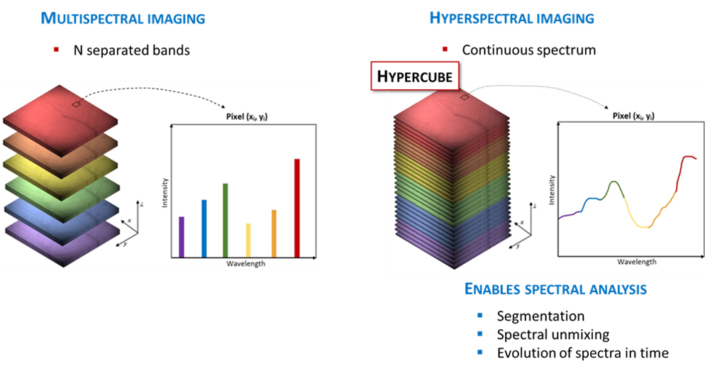
\includegraphics[width=0.7\linewidth]{media/images/hyperspectral_image.png}
    \caption{Esquemas para almacenar los valores de píxel reales de una imagen en un archivo \acrshort{bil}, referencia: \cite{Archivos82:online}}
    \label{fig:hyperspectral_image}
\end{figure}

\begin{code}[numbers=left]{title=Gráfico de velas de los outliers, label=code:plot-outliers}{Python}
def plots_outliers(outliers_df: pd.DataFrame, column=53):
    fig, axes = plt.subplots(ncols=2, figsize=(10, 5))
    sns.histplot(outliers_df[column], binwidth=1, ax=axes[0])
    sns.boxplot(outliers_df[column], ax=axes[1])
    fig.tight_layout()
    plt.show()
\end{code}

\begin{code}[numbers=left]{title=Detección de outliers utilizando \textit{zscore}, label=code:zscore}{Python}
...
    zscore = np.abs(stats.zscore(df))
    data_clean = df[(zscore < 3).all(axis=1)]
    df = data_clean
...
\end{code}

\begin{code}[numbers=left]{title=Gráfico de curvas de aprendizaje, label=code:plot-learning-curves}{Python}
def plots_balancing(df, df_balanced):
    fig, axis = plt.subplots(ncols=2, figsize=(10, 5))
    fig.suptitle(f'Balance of {src.utils.dev_config.OBJECTIVE_COLUMN}')
    axis[0].set_title(f'Before balancing {src.utils.dev_config.OBJECTIVE_COLUMN}')
    axis[1].set_title(f'After balancing {src.utils.dev_config.OBJECTIVE_COLUMN}')
    plot_balance(df, ax, 0)
    plot_balance(df_balanced, ax, 1)
    f.tight_layout()
    plt.show()
z

def plot_balance(df, axis, axis_number):
    return sns.histplot(df[src.utils.dev_config.OBJECTIVE_COLUMN], ax=axis[axis_number] if axis_number else axis)
\end{code}

\begin{code}[numbers=left]{title=Gráfico de comparación del balanceo, label=code:plots_balancing}{Python}
def plot_learning_curves(model, model_name, x, y):
    x_train, x_val, y_train, y_val = train_test_split(x, y, test_size=0.2)
    train_errors, val_errors = [], []
    
    for m in range(5, len(x_train)):
        model.fit(x_train[:m], y_train[:m])
        y_train_predict = model.predict(x_train[:m])
        y_val_predict = model.predict(x_val)
        train_errors.append(metrics.fbeta_score(y_train[:m], y_train_predict, beta=2))
        val_errors.append(metrics.fbeta_score(y_val, y_val_predict, beta=2))
        
    plt.title(f'{model_name} - Learning curves')
    plt.plot(np.sqrt(train_errors), "r-+", linewidth=2, label="train")
    plt.plot(np.sqrt(val_errors), "b-", linewidth=3, label="val")
    plt.xlabel("Training set size")
    plt.ylabel("f2 score")
    plt.legend(loc="best")
    plt.show()
\end{code}

% ---------------------------------------------------------- %
% 
\clearpage

% APPENDIX
% \subfile{sections/appendix}
% \clearpage

% SPECIAL TERMS
\printglossary[title=Definiciones adicionales, nonumberlist]
\label{sec:additional-definitions}
\clearpage

% BIBLIOGRAPHY
\printbibliography[heading=bibintoc, title=Bibliografía y referencias]


\end{document}